%(BEGIN_QUESTION)
% Copyright 2011, Tony R. Kuphaldt, released under the Creative Commons Attribution License (v 1.0)
% This means you may do almost anything with this work of mine, so long as you give me proper credit

Anta at du har en strøm-til-trykk-omformer (``I/P'') med et utgangsområde på 3 til 15 PSI og et inngangsområde på 4 til 20 mA. Følgende kalibreringstabell viser flere nivåer for inngangssignalet og tilhørende prosent av spenn og utgangstrykk:

% No blank lines allowed between lines of an \halign structure!
% I use comments (%) instead, so that TeX doesn't choke.

$$\vbox{\offinterlineskip
\halign{\strut
\vrule \quad\hfil # \ \hfil & 
\vrule \quad\hfil # \ \hfil & 
\vrule \quad\hfil # \ \hfil \vrule \cr
\noalign{\hrule}
%
% First row
Påført inngangssignal & Prosent av spenn & Utgangstrykk \cr
%
% Another row
(mA) & (\%) & (PSI) \cr
%
\noalign{\hrule}
%
% Another row
6.88 & 18 & 5.16 \cr
%
\noalign{\hrule}
%
% Another row
5.1 & 6.88 & 3.83 \cr
%
\noalign{\hrule}
%
% Another row
12.8 & 55 & 9.6 \cr
%
\noalign{\hrule}
%
% Another row
17.44 & 84 & 13.08 \cr
%
\noalign{\hrule}
%
% Another row
6.53 & 15.83 & 4.9 \cr
%
\noalign{\hrule}
} % End of \halign 
}$$ % End of \vbox

Selv om beregningene for å få prosent og utgangstrykk (PSI) fra inngangsstrøm (mA) ikke er spesielt kompliserte, kan de være tidkrevende. Et kraftig databasert verktøy for å redusere dette arbeidet er en type program som kalles et {\it regneark}. Et svært vanlig eksempel på regnearkprogramvare er Microsoft {\it Excel} (selv om det finnes andre regnearkprogrammer, noen av dem gratis!).

Et regnearkprogram viser en skjerm full av rektangulære {\it celler} der tekst, tallverdier og matematiske formler kan legges inn. Hver celle har en ``adresse'' basert på rad- og kolonnekoder, tradisjonelt tall for rader og bokstaver for kolonner (som i spillet ``Battleship'' der koordinater på et rutenett oppgis med bokstav og tall), men en nyere konvensjon angir både rader og kolonner med tall.

Vi kan sette opp et regneark til å beregne prosentverdier for denne I/P-en basert på inngangsstrømmer slik. Gul og blå cellefylling vist i eksemplet er helt valgfritt, men gjør det lettere å skille mellom felt for tallinnskriving og felt med beregnede verdier (tallet i den gule cellen {\tt R2C1} er milliamp-verdien du skriver inn i regnearket, mens tallet i den blå cellen {\tt R2C3} er PSI-verdien som regnearket beregner):

$$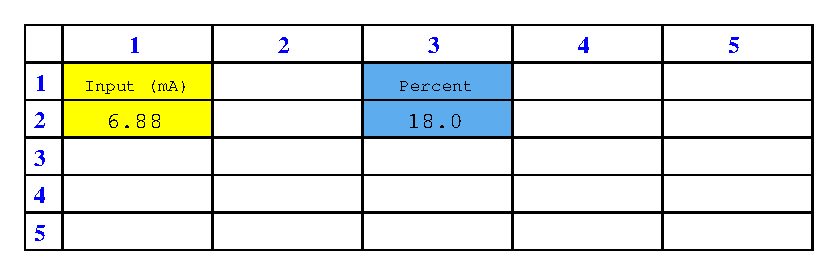
\includegraphics[width=15.5cm]{i01626x01.eps}$$

Følgende er en liste over celleinnhold som trengs for å lage regnearket du ser over:

\begin{itemize}
\item{} {\bf Celle R1C1:} {\tt Input (mA)}
\item{} {\bf Celle R2C1:} {\tt 6.88}
\item{} {\bf Celle R1C3:} {\tt Percent}
\item{} {\bf Celle R2C3:} {\tt = (R2C1 - 4) / 16} \hskip 10pt {\it (velg visningsformat ``\%'')}
\end{itemize}

Teksten i cellene R1C1 og R1C3 er ikke nødvendig for at regnearket skal fungere -- akkurat som fargefyllingen fungerer den bare som etiketter som forklarer hva tallverdiene betyr. Formelen som legges inn i celle R2C3 begynner med et likhetstegn (=), som forteller regnearket at dette er en formel og ikke ren tekst slik som i R1C1 og R1C3. Merk hvordan formelen refererer til tallverdien i cellen ``rad 2 kolonne 1'' ved å kalle den ``R2C1''. Dette gjør at brukeren kan legge inn ulike verdier i celle R2C1, og regnearket vil automatisk beregne prosentverdien på nytt for hver mA-verdi som legges inn. Hvis du for eksempel endrer innholdet i celle R2C1 fra 6.88 til 12.8, vil verdien vist i celle R2C3 oppdateres fra 18.0 til 55.0.

\vskip 10pt

\vfil \eject

Din første oppgave her er å starte et regnearkprogram og legge inn det som er vist over, og deretter validere at arbeidet ditt er riktig ved å legge inn flere ulike strømverdier (milliamp) og kontrollere at prosentverdiene beregnes korrekt av regnearket.

Nå som du har laget dette regnearket, legg inn passende verdier i cellene R1C5 og R2C5 slik at det også beregner riktig utgangstrykk for I/P-en, for en vilkårlig inngangsstrøm som legges inn i celle R2C1. Når du er ferdig, skal det endrede regnearket se omtrent slik ut:

$$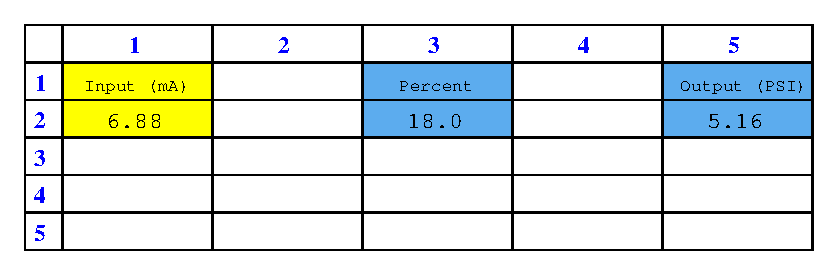
\includegraphics[width=15.5cm]{i01626x02.eps}$$

Vis hvilke innskrivinger du måtte legge inn i cellene R1C5 og R2C5 for at regnearket skal fungere.

\vskip 20pt \vbox{\hrule \hbox{\strut \vrule{} {\bf Forslag til sokratisk diskusjon} \vrule} \hrule}

\begin{itemize}
\item{} Identifiser tegnet som brukes for å representere {\it divisjon} i formelen i celle R2C3. Hvilket tegn brukes for {\it multiplikasjon}?
\item{} Forklar hvorfor parenteser brukes i formelen i celle R2C3. {\it Hint: en god problemløsningsmetode er å analysere hva som ville skjedd hvis parentesene ikke var der!}
\item{} Forklar hva som ville skjedd dersom celle R2C3 ikke var satt opp til å vises som {\it prosent}.
\item{} Det finnes mer enn én riktig formel å legge inn i celle R2C5 for korrekt beregning av utgangstrykk i PSI. Én formel refererer prosentverdien (i R2C3), mens den andre refererer milliamp-verdien (i R2C1). Sammenlign disse to formlene, og forklar hvilken som gir mest mening for deg.
\item{} Forklar hvorfor et regneark er et så kraftig matematisk verktøy for å utføre ``tidkrevende'' beregninger som instrumenters inn-/utgangsresponser. Kommer du på andre praktiske bruksområder for et regneark?
\end{itemize}

\underbar{file i01626}
%(END_QUESTION)





%(BEGIN_ANSWER)

Her er to mulige formler for innlegging i celle R2C5:

\vskip 10pt

{\tt = ((R2C1 - 4) / 16) * 12 + 3}

\vskip 10pt

{\tt = R2C3 * 12 + 3}

\vskip 10pt

Én svært praktisk bruk av denne typen regnearkprogram er å lage øvingsoppgaver til seg selv, slik at man kan øve på beregning av instrumenters inn-/utgangsområder.

%(END_ANSWER)





%(BEGIN_NOTES)

\vfil \eject

\noindent
{\bf Oppsummeringsquiz:}

Beregn utgangstrykket (område 3-15 PSI) fra en I/P-omformer med et inngangssignal på 13 mA (område 4-20 mA):

\begin{itemize}
\item{} 13.0 PSI
\vskip 5pt
\item{} 12.75 PSI
\vskip 5pt
\item{} 10.8 PSI
\vskip 5pt
\item{} 9.75 PSI
\vskip 5pt
\item{} 13.4 PSI
\vskip 5pt
\item{} 17.33 PSI
\end{itemize}

%INDEX% Calibration: table, I/P transducer
%INDEX% Computer spreadsheet exercise: introduction to spreadsheet usage
%INDEX% Computer spreadsheet exercise: I/P transducer input/output calculations

%(END_NOTES)
